\begin{figure}[!htb]

    \centering

    \begin{subfigure}[b]{0.49\textwidth}
        \centering
        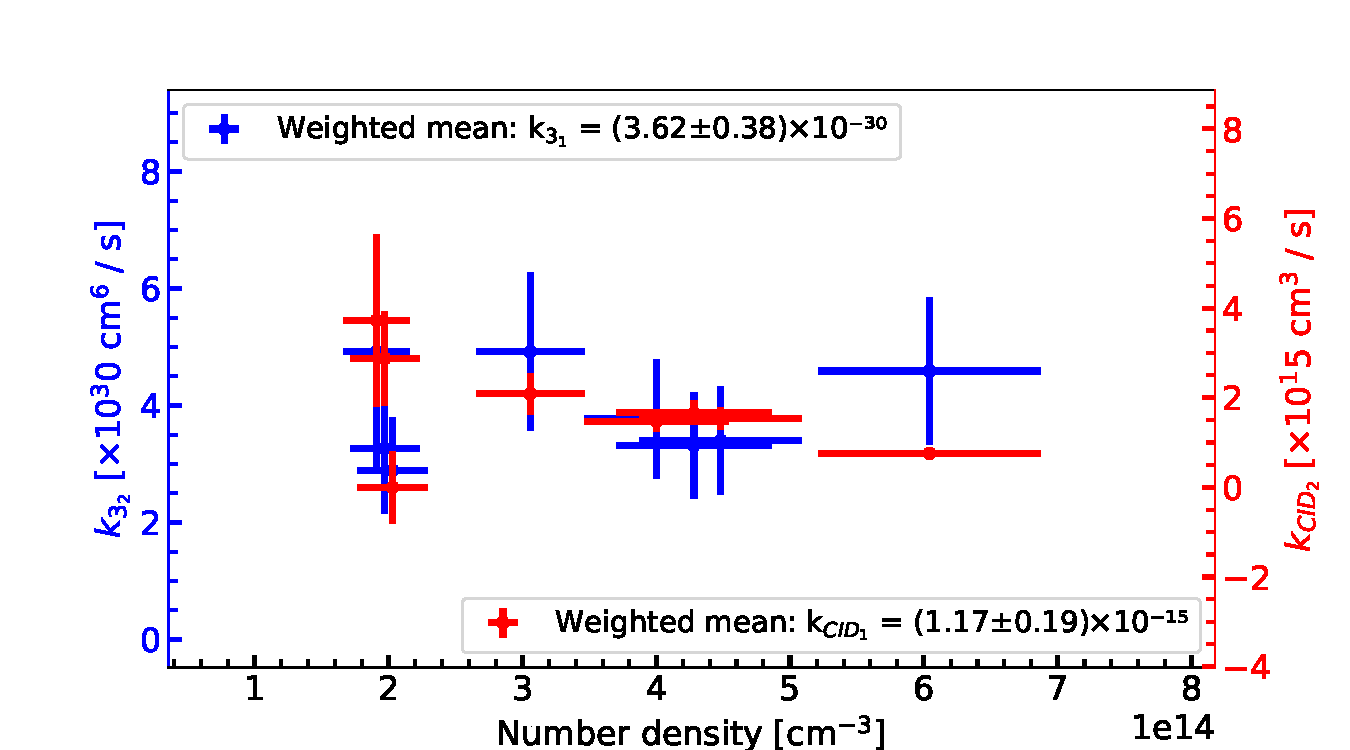
\includegraphics[width=1\textwidth]{figures/measurements/kinetics/rate-constants-higher-order/off_4.8K_k3_kCID_2_as_functionOfnHe.pdf}
        \caption{}
        
    \end{subfigure}
    \hfill
    \begin{subfigure}[b]{0.49\textwidth}
        \centering
        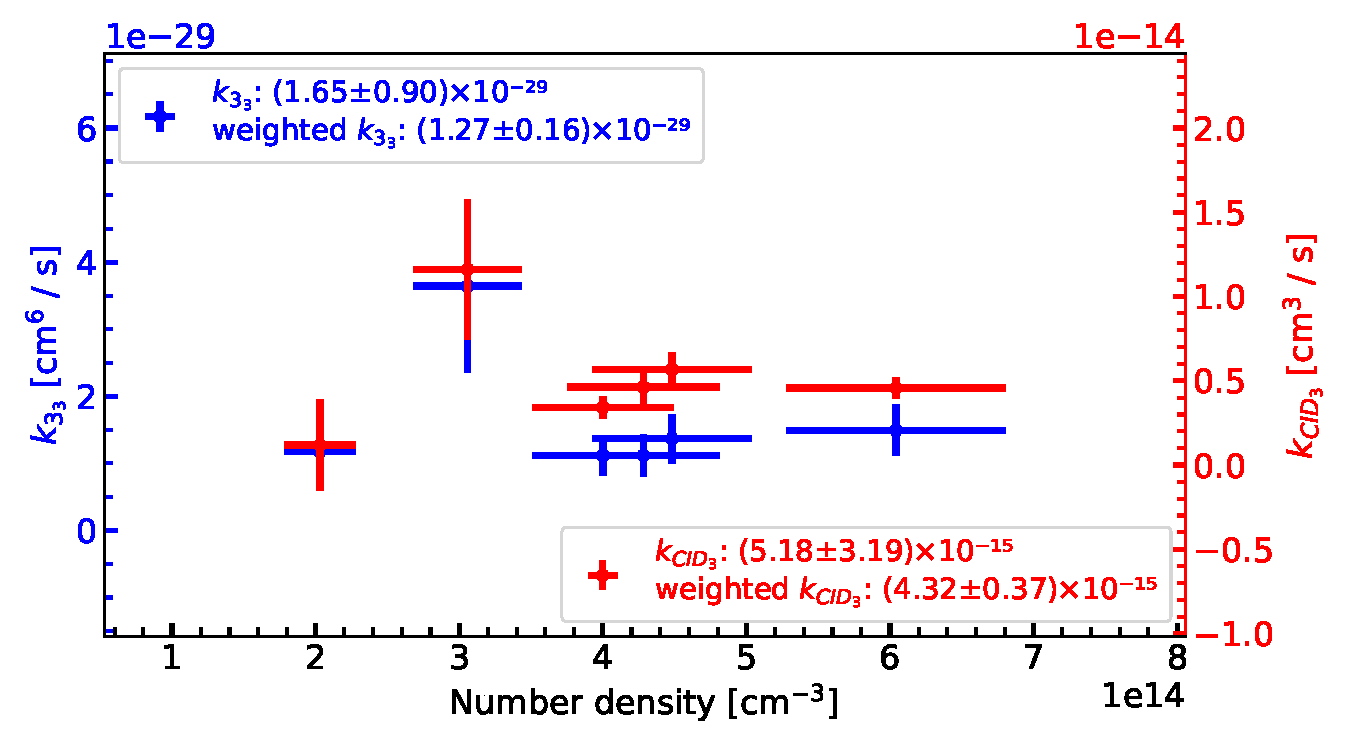
\includegraphics[width=1\textwidth]{figures/measurements/kinetics/rate-constants-higher-order/off_4.8K_k3_kCID_3_as_functionOfnHe.pdf}
        \caption{}
        
    \end{subfigure}
    
    \begin{subfigure}[b]{0.49\textwidth}
        \centering
        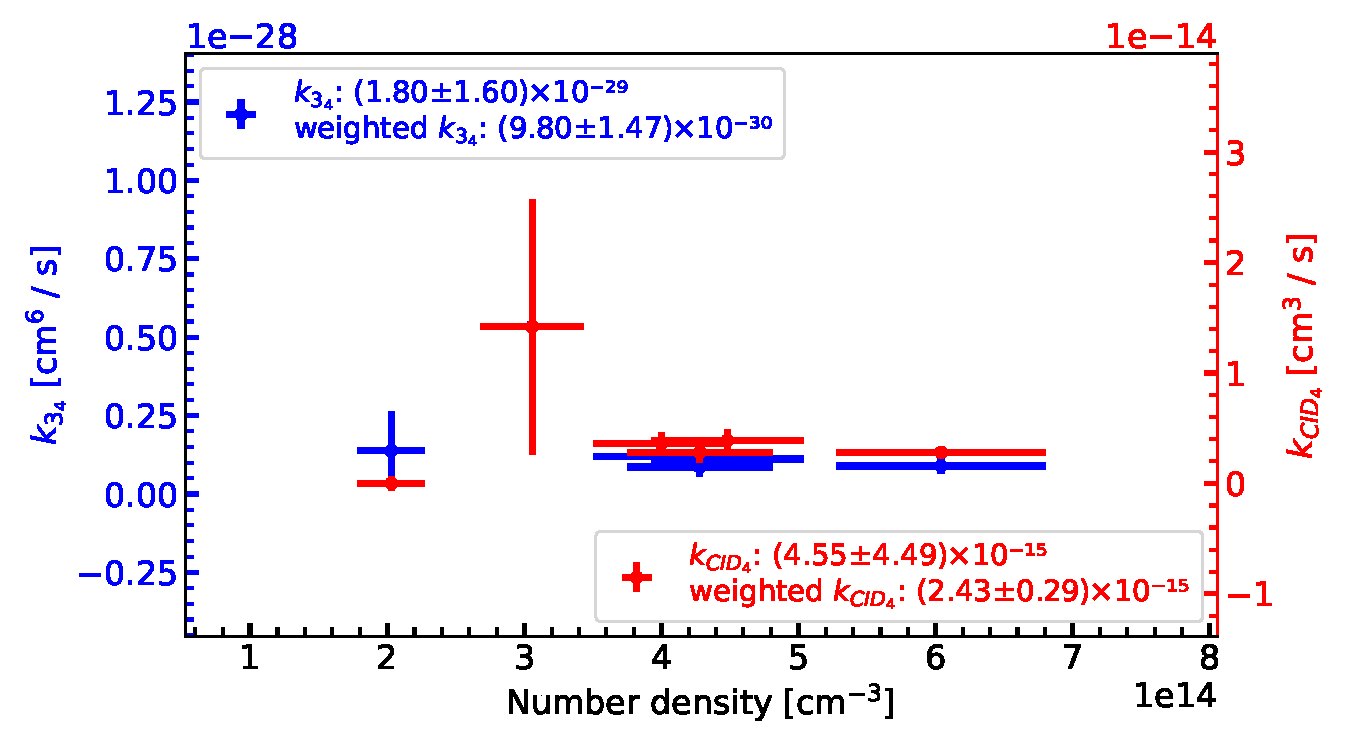
\includegraphics[width=1\textwidth]{figures/measurements/kinetics/rate-constants-higher-order/off_4.8K_k3_kCID_4_as_functionOfnHe.pdf}
        \caption{}
        
    \end{subfigure}
    \hfill
    \begin{subfigure}[b]{0.49\textwidth}
        \centering
        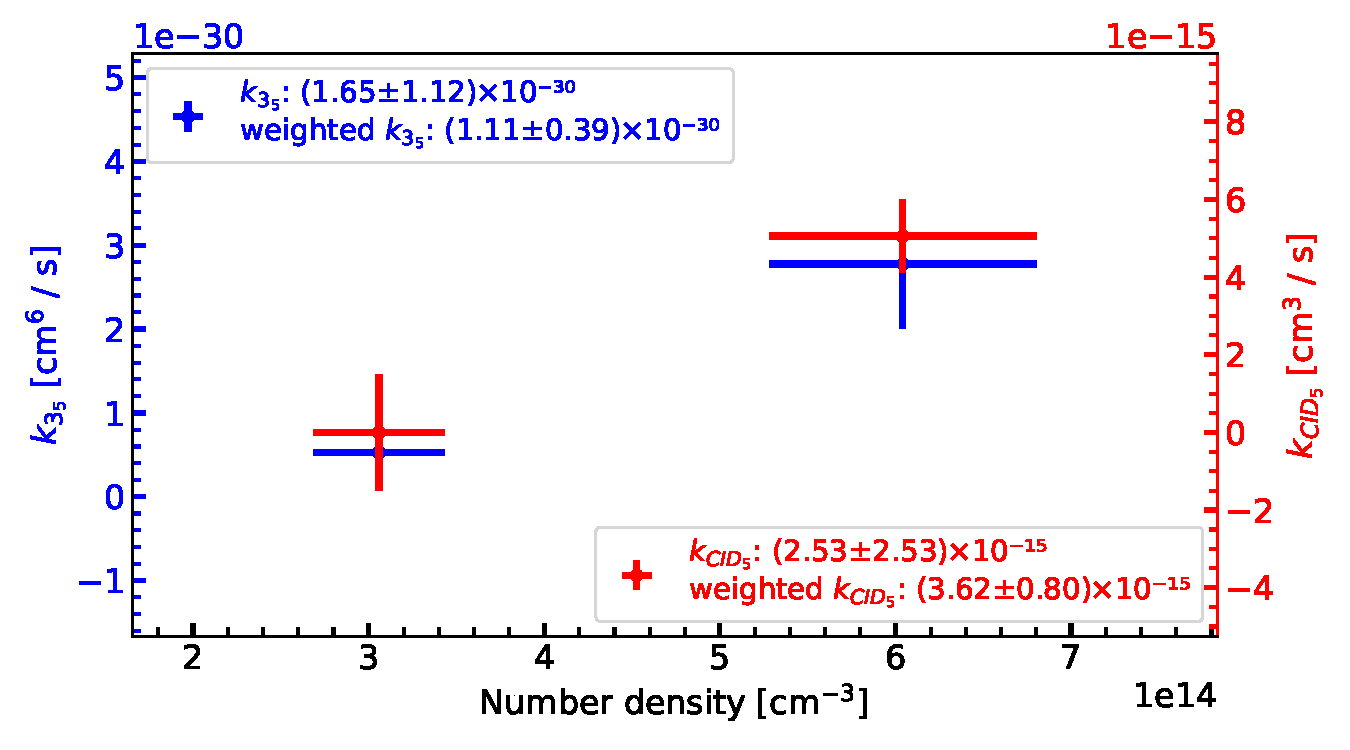
\includegraphics[width=1\textwidth]{figures/measurements/kinetics/rate-constants-higher-order/off_4.8K_k3_kCID_5_as_functionOfnHe.pdf}
        \caption{}
        
    \end{subfigure}
    
    \caption{The numerically derived formation and dissociation rate constants for higher order of complexes $(n>1)$ plotted as a function of number density at 4.8(3) K temperature.}
    \label{fig:rate-constants-higher-order}

\end{figure}